\EXERCISE
نقشه‌ی زیر محل ایران و توران را نشان می‌دهد. رستم قصد دارد ارتش خود را از ایران به سمت توران حرکت دهد. ارتش او هر روز می‌تواند به اندازه‌ی یک واحد روی نقشه حرکت کند. اگر او
$10$
روز وقت داشته باشد تا ارتش را به توران برساند، تعداد روش‌های حرکت ارتش برای رسیدن به توران را تحت شرایط زیر بیابید:
\begin{enumerate}
\item
ارتش حتما از بخارا عبور کند.
\item
ارتش از بلخ عبور کند اما از سمرقند عبور نکند.
\end{enumerate}
\begin{center}
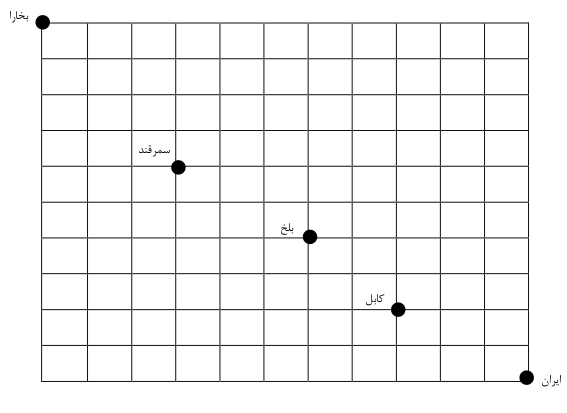
\includegraphics[height=6.5cm]{13.png}
\end{center}